 \documentclass[a4paper,12pt]{article}
\usepackage[a4paper,top=1.3cm,bottom=2cm,left=1.5cm,right=1.5cm,marginparwidth=0.75cm]{geometry}
\usepackage{setspace}
\usepackage{cmap}					
\usepackage{mathtext} 				
\usepackage[T2A]{fontenc}			
\usepackage[utf8]{inputenc}			
\usepackage[english,russian]{babel}
\usepackage{multirow}
\usepackage{graphicx}
\graphicspath{ {./images/} }
\usepackage{wrapfig}
\usepackage{tabularx}
\usepackage{float}
\usepackage{longtable}
\usepackage{hyperref}
\hypersetup{colorlinks=true,urlcolor=blue}
\usepackage[rgb]{xcolor}
\usepackage{amsmath,amsfonts,amssymb,amsthm,mathtools} 
\usepackage{icomma} 
\mathtoolsset{showonlyrefs=true}
\usepackage{euscript}
\usepackage{mathrsfs}

\DeclareMathOperator{\sgn}{\mathop{sgn}}
\newcommand*{\hm}[1]{#1\nobreak\discretionary{}
	{\hbox{$\mathsurround=0pt #1$}}{}}

\title{\textbf{Исследование прецессии уравновешенного гироскопа (1.2.5)}}
\author{Павлушкин Вячеслав}
\date{December 2021}


\begin{document}
	
	\maketitle
	
	\section{Введение}
	
	\textbf{Цель работы:} исследовать вынужденную прецессию гироскопа, установить зависимость скорости вынужденной прецессии от величины момента сил, действующий на ось гироскопа и сравнить ее со скоростью, рассчитанной по скорости прецессии.\\
	\textbf{Оборудование:} гироскоп в кардановом подвесе, секундомер, набор грузов, отдельный ротор гироскопа, цилиндр известной массы, крутильный маятник, штангенсциркуль, линейка.
	
	\section{Теоретические сведения}
	
	В этой работе исследуется зависимость скорости прецессии гироскопа от момента силы, приложенной к его оси. Для этого к оси гироскопа подвешиваются грузы. Скорость прецессии определяется по числу оборотов рычага вокруг вертикальной оси и времни, которое на это ушло, определяемоу секундомером. В процессе измерений рычаг не только поворачивается в результате прецессии гироскопа, но и опускается. Поэтому его в начале опыта следует преподнять на 5-6 градусов.  Опять надо закончить, когда рычаг опустится на такой же угол.\\
	\begin{center}$
		\begin{array}{cc}
			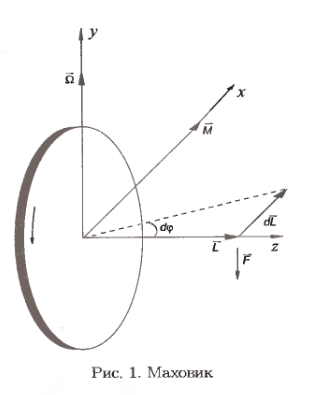
\includegraphics[width=0.40\textwidth]{img1.png}&
			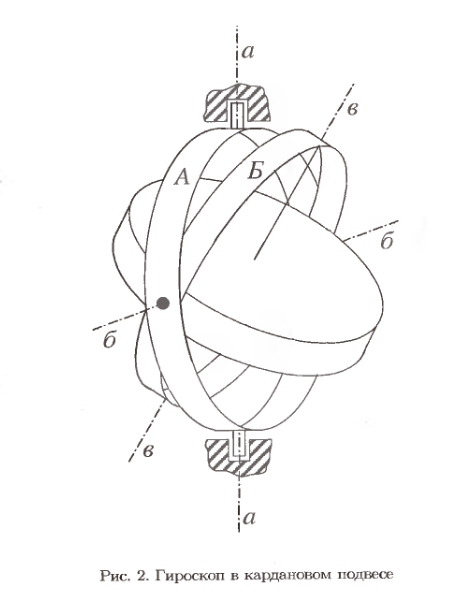
\includegraphics[width=0.40\textwidth]{img2.png}\\
		\end{array}$
	\end{center}
	
	Измерение скорости прецессии гироскопа позволяет вычислить угловую скорость вращения его ротора. Расчет производится по формуле:
	
	\begin{equation}
		\Omega = \frac{mgl}{I_z\omega_0},
	\end{equation}
	
	где $m$ -- масса груза, $l$ -- расстояние от центра карданова подвеса до точки крепления груза на оси гироскопа, $I_z$ -- момент инерции гироскопа по его главной оси вращения. $\omega_0$ -- частота его вращения относительно главной оси, $\Omega$ -- частота прецессии.\\
	Момент инерции ротора относительно оси симметрии $I_0$ измеряется по крутильным колебаниям точной копии ротора, подвешиваемой вдоль оси симметрии на десткой проволоке. Период крутильных колебаний $T_0$ зависит от момента инерции $I_0$ и модуля кручения проволоки $f$:
	
	\begin{equation}
		T_0 = 2\pi\sqrt{\frac{I_0}{f}}.
	\end{equation}
	
	Чтобы исключить модуль кручения проволоки, вместо ротора гироскопа к той же проволоке подвешивают цилиндр правильной формы с известными размерами и массой, для которого легко можно вычислить момент инерции $I_\text{ц}$. Для определения момента инерции ротора гироскопа имеем:
	
	\begin{equation}
		I_0 = I_\text{ц}\frac{T_0^2}{T_\text{ц}^2},
		\label{moment}
	\end{equation}
	Здесь $T_\text{ц}$ -- период крутильных колебаний цилиндра.\\
	\begin{center}
		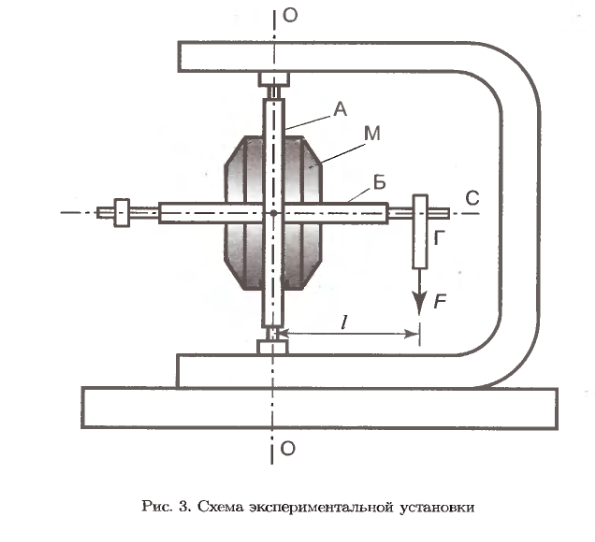
\includegraphics[width=0.8\textwidth]{img3.png}
	\end{center}
	
	Скорость вращения ротора гироскопа можно определить и не прибегая к исследованию прецессии. У используемых в работе гироскопов статор имеет две обмотки, необходимые для быстрой раскрутки гироскопа. В данной работе одну обмотку искользубт для раскрутки гироскопа, а вторую -- для измерения числа оборотов ротора. Ротор электромотора всегда немного намагничен. Вращаясь, он наводит во второй обмотке переменную ЭДС индукции, частота которой равна частоте врещения ротора. Частоту этой ЭДС можно, в частности, измерить по фигурам Лиссажу, получаемым на экране осциллографа, если на один вход подать исследуемую ЭДС, а на другой -- переменное напряжение с хорошо прокалиброванного генератора. При совпадении частот на эеране получаем эллипс.
	
	\section{Ход работы}
	Данные для частоты прецессии и опускания гироскопа: $\Omega=\frac{2\pi N}{t}$
	
	\begin{center}
		\begin{tabular}{|c|c|c|c|}
			\hline
			Масса & $T$, с& $N$ & $\Omega$, $\text{с}^{-1}$  \\
			\hline
			\multirow{2}{*}{$m = 336$ г}&178,52&6&21,12$\cdot 10^{-2}$ \\
			\cline{2-4}
			&179,23 & 6 &21,03$\cdot 10^{-2}$  \\
			\hline
		\end{tabular}
		\quad
		\begin{tabular}{|c|c|c|c|}
			\hline
			Масса & $T$, с& $N$ & $\Omega$, $\text{с}^{-1}$ \\
			\hline
			\multirow{2}{*}{$m = 269$ г}&186,41&5&16,85$\cdot 10^{-2}$ \\
			\cline{2-4}
			&187,02 & 5 &16,80$\cdot 10^{-2}$  \\
			\hline
		\end{tabular}
	\end{center}
	
	\begin{center}
		\begin{tabular}{|c|c|c|c|}
			\hline
			Масса & $T$, с& $N$ &$\Omega$, $\text{с}^{-1}$ \\
			\hline
			\multirow{2}{*}{$m = 215$ г}&188,31&4& 13,35$\cdot 10^{-2}$ \\
			\cline{2-4}
			&188,01 & 4 &13,38$\cdot 10^{-2}$  \\
			\hline
		\end{tabular}
		\quad
		\begin{tabular}{|c|c|c|c|}
			\hline
			Масса & $T$, с& $N$ &$\Omega$, $\text{с}^{-1}$ \\
			\hline
			\multirow{2}{*}{$m = 174$ г}&232,43&4&10,81$\cdot 10^{-2}$ \\
			\cline{2-4}
			&231,07 & 4 &10,88$\cdot 10^{-2}$  \\
			\hline
		\end{tabular}
	\end{center}
	
	\begin{center}
		\begin{tabular}{|c|c|c|c|}
			\hline
			Масса & $T$, с& $N$ &$\Omega$, $\text{с}^{-1}$ \\
			\hline
			\multirow{2}{*}{$m = 138$ г}&219,81&3&8,58$\cdot 10^{-2}$ \\
			\cline{2-4}
			&218,99 & 3 &8,61$\cdot 10^{-2}$  \\
			\hline
		\end{tabular}
	\end{center}
	
	Каждый раз рычаг опускался на $12^\circ$, что равняется $\dfrac{\pi}{15}$. Для каждой массы посчитаем угловую скорость опускания рычага по формуле: $\omega = \dfrac{\pi/15}{T}$, и момент $M = mgl$, где $l = 121$ мм:
	\begin{itemize}
		\item $m = 336$ г, $\omega = 11,71\cdot 10^{-4}$ $\text{с}^{-1}$, $M = 39,88\cdot10^{-2}$ Н$\cdot$м
		\item $m = 269$ г, $\omega = 11,22\cdot 10^{-4}$ $\text{с}^{-1}$, $M = 31,93\cdot10^{-2}$ Н$\cdot$м
		\item $m = 215$ г, $\omega = 11,13\cdot 10^{-4}$ $\text{с}^{-1}$, $M = 25,52\cdot10^{-2}$ Н$\cdot$м
		\item $m = 174$ г, $\omega = 9,04\cdot 10^{-4}$ $\text{с}^{-1}$, $M = 20,65\cdot10^{-2}$ Н$\cdot$м
		\item $m = 138$ г, $\omega = 9,55\cdot 10^{-4}$ $\text{с}^{-1}$, $M = 16,38\cdot10^{-2}$ Н$\cdot$м
	\end{itemize}
	
	Построим график зависимости $\Omega(M)$:
	\begin{figure}[h!]
		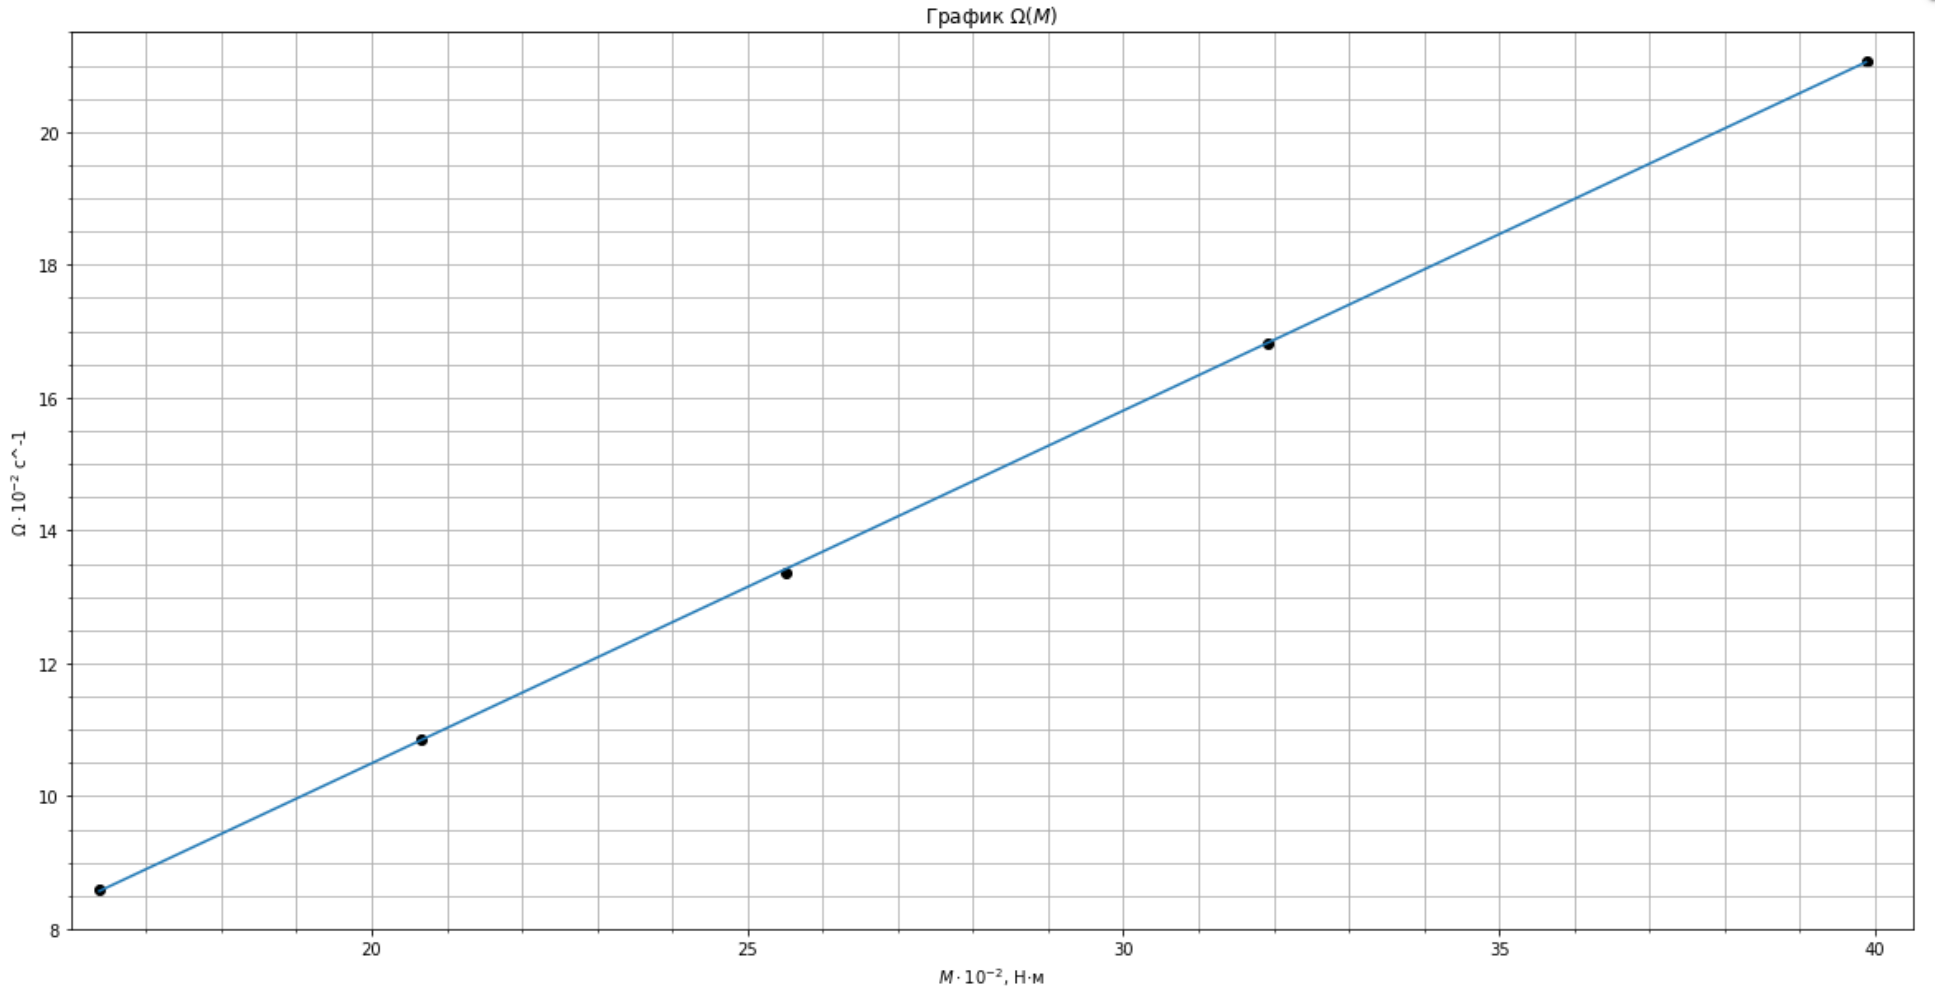
\includegraphics[scale=0.53]{1.2.5 graph}
		\caption{Зависимость $ \Omega $ от $ M $}
		\label{graph}
	\end{figure}

	Далее найдем момент инерции ротора гироскопа по формуле \eqref{moment}, для этого посчитаем момент инерции цилиндра, с известной нам массой и диаметром: $I_\text{ц} = \dfrac{1}{2}mr^2 \approx 1,23\cdot 10^{-3}$ кг$\cdot \text{м}^2$, а периоды: $T_0 = 3,933$ с и $T_\text{ц} = 3,19$ с. Тогда $I_0 \approx 0,8\cdot 10^{-3}$ кг$\cdot \text{м}^2$
	
	\section{Погрешности $\Omega$ и $I_0$}
	
	\begin{equation}
		\sigma_\Omega = \sqrt{ \sigma_\text{случ}^2 + \sigma_\text{сист}^2} \;\;\;\;\;\; \sigma_\Omega^\text{сист} = \Omega \varepsilon_T \;\;\;\;\;\; \sigma_\Omega^\text{случ}=  \sqrt{\frac{1}{n(n-1)} \sum_{i=1}^{n}(\Omega_i - \overline{\Omega})^2}
	\end{equation}
	
	Каждая частота $\Omega$ с учетом погрешностей:
	\begin{itemize}
		\item $\Omega = (21,08 \pm 0,03)\cdot10^{-2}\text{ }\text{с}^{-1}$ 
		\item $\Omega = (16,83 \pm 0,04)\cdot10^{-2}\text{ }\text{с}^{-1}$
		\item $\Omega = (13,37 \pm 0,05)\cdot10^{-2}\text{ }\text{с}^{-1}$
		\item $\Omega = (10,85 \pm 0,05)\cdot10^{-2}\text{ }\text{с}^{-1}$
		\item $\Omega = (8,60 \pm 0,03)\cdot10^{-2}\text{ }\text{с}^{-1}$
	\end{itemize}

	Погрешность $\sigma_{I_0} = I_0\cdot\sqrt{\varepsilon_{I_\text{ц}}^2+ 4\varepsilon_{T_0}^2+ 4\varepsilon_{T_\text{ц}}^2 } \approx 0,03$ кг$\cdot \text{м}^2$, значит $I_0 = (0,80\pm 0,03)$ кг$\cdot \text{м}^2$
	
	\section{Определение частоты вращения ротора гироскопа}
	
	Определить частоту вращения ротора можно по формуле $\omega_0 = \dfrac{1}{kI_0}$, где $k$ -- коэффицент наклона графика зависимости $\Omega(M)$.
	
	График построен по МНК, а значит:
	\begin{equation}
	k=\frac{\langle xy\rangle-\langle x\rangle \langle y\rangle}{\langle x^2\rangle - \langle x\rangle^2}\approx 0,531\text{ }\frac{1}{\text{Дж}\cdot\text{с}}
	\end{equation}
	\begin{equation}
		\sigma_k^\text{сл}=\frac{1}{\sqrt{N}}\sqrt{\frac{\langle y^2 \rangle - \langle y \rangle^2}{\langle x^2 \rangle - \langle x \rangle^2} - k^2  } \approx 0,002\text{ }\frac{1}{\text{Дж}\cdot\text{с}}
	\end{equation}

	Тогда $\omega_0 = 2354,05\text{ }\text{с}^{-1}$, а $\sigma_{\omega_0} = \omega_0\cdot\sqrt{\varepsilon_{I_0}^2+ \varepsilon_k^2} \approx 88,72\text{ }\text{с}^{-1}$
	
	Используя полученную угловую скорость можно определить частоту вращения ротора гироскопа: $\nu = \dfrac{\omega_0}{2\pi} \approx 374,7\text{ }\text{Гц}$, а $\sigma_{\nu} = \nu\varepsilon_{\omega_0} \approx 14,1\text{ }\text{Гц}$
	
	Таким образом получаем: \underline{$\nu = (374,7\pm14,1)\text{ Гц}$}, что с учетом сигмы попадает в значение полученное с помощью осциллографа $\nu_0 = 387,2\text{ Гц}$
	
	\section{Момент силы трения}
	
	Оценить момент силы трения мы можем по формуле: $M = \omega I_0 \omega_0$, а $\sigma_M = M\cdot\sqrt{\varepsilon_M^2+ \varepsilon_k^2}$. Для каждой массы момент силы трения будет свой:
	
	\begin{itemize}
		\item $m = 336$ г, $\omega = 11,71\cdot 10^{-4}$ $\text{с}^{-1}$, $M = (2,21\pm0,02)\cdot10^{-3}$ Н$\cdot$м
		\item $m = 269$ г, $\omega = 11,22\cdot 10^{-4}$ $\text{с}^{-1}$, $M = (2,11\pm0,02)\cdot10^{-3}$ Н$\cdot$м
		\item $m = 215$ г, $\omega = 11,13\cdot 10^{-4}$ $\text{с}^{-1}$, $M = (2,09\pm0,02)\cdot10^{-3}$ Н$\cdot$м
		\item $m = 174$ г, $\omega = 9,04\cdot 10^{-4}$ $\text{с}^{-1}$, $M = (1,70\pm 0,02)\cdot10^{-3}$ Н$\cdot$м
		\item $m = 138$ г, $\omega = 9,55\cdot 10^{-4}$ $\text{с}^{-1}$, $M = (1,80 \pm 0,02)\cdot10^{-3}$ Н$\cdot$м
	\end{itemize}  

	
\end{document}